Dalle nostre specifiche emerge che la nostra base di dati si occuper� principalmente delle interazioni dei Personaggi all'interno del gioco, a partire da questa, dovremo quindi stabilire le entit� principali all'interno del gioco.
Sappiamo che nel Gioco incontreremo sia personaggi che NPC.

\begin{figure}[H]
\centering
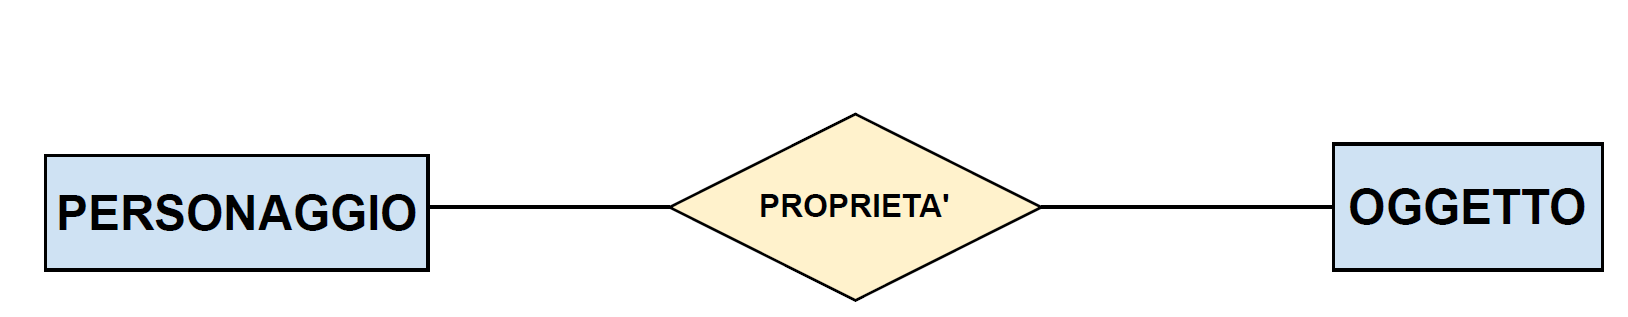
\includegraphics[width=0.7\linewidth]{./immagini/PERSONAGGIOPROPROGETTO.png}
\end{figure}



Gli Oggetti di propriet� del personaggio rappresentano una entit� molto importante, essi possono appartenere anche a un NPC

\begin{figure}[H]
\centering
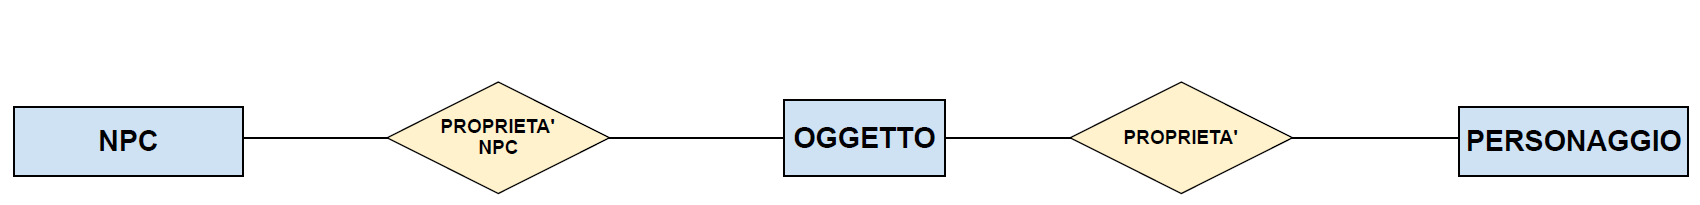
\includegraphics[width=0.7\linewidth]{./immagini/oggettotriplo.png}
\end{figure}


All'interno del gioco il personaggio interagisce con altri personaggi ed NPC come descritto nello schema dei processi interni, 
sappiamo che le interazioni di combattimento sono gestite dal Programma e non interessano la Base di Dati, tuttavia una interazione fondamentale �
la Transazione, in quanto ogni personaggio pu\`{o} vendere oggetti ad un altro o ad un NPC e risulta necessario tenere traccia di queste TRANSAZIONI

I personaggi Intraprendono e completano MISSIONI necessarie all'avanzamento nel gioco

\begin{figure}[H]
\centering
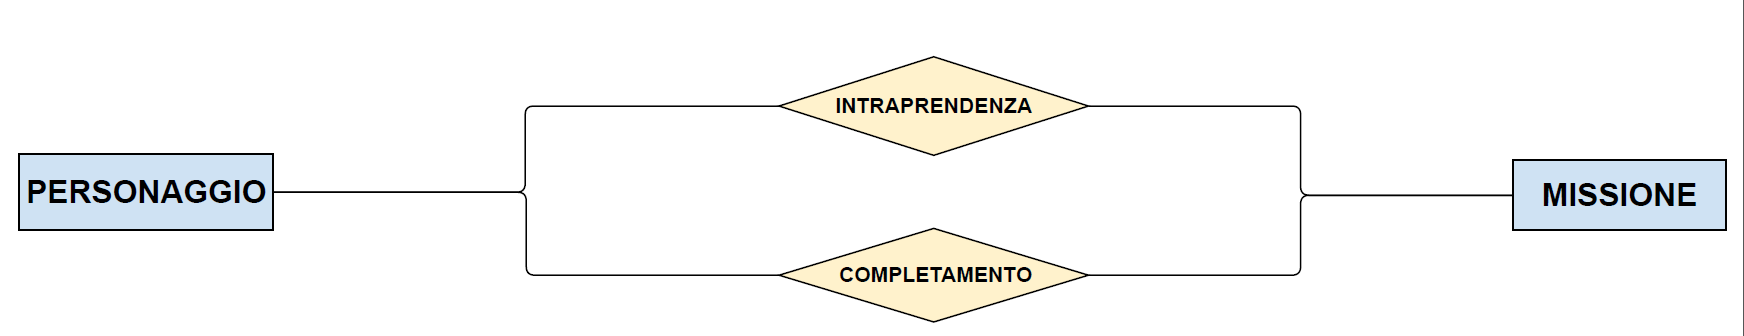
\includegraphics[width=0.7\linewidth]{./immagini/persomiss.png}
\end{figure}


Essi possono inoltre apprendere delle abilit� da degli NPC che le insegnano in cambio di denaro

\begin{figure}[H]
\centering
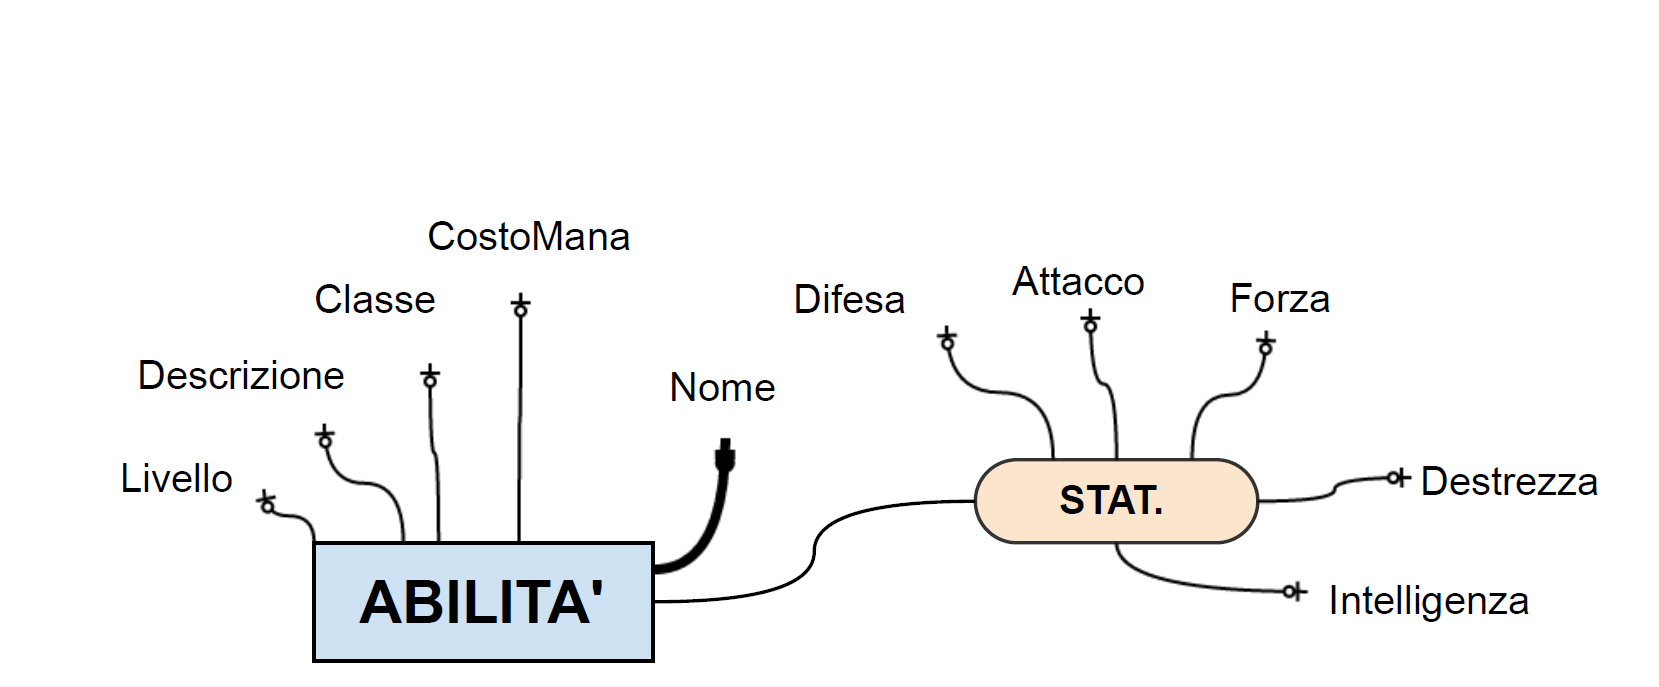
\includegraphics[width=0.7\linewidth]{./immagini/ABILITADEF.png}
\end{figure}

All'esterno del gioco vero e proprio sappiamo che ci� che accade � principalmente la creazione di personaggi dell'utente e l'acquisto di prodotti dallo store

\begin{figure}[H]
\centering
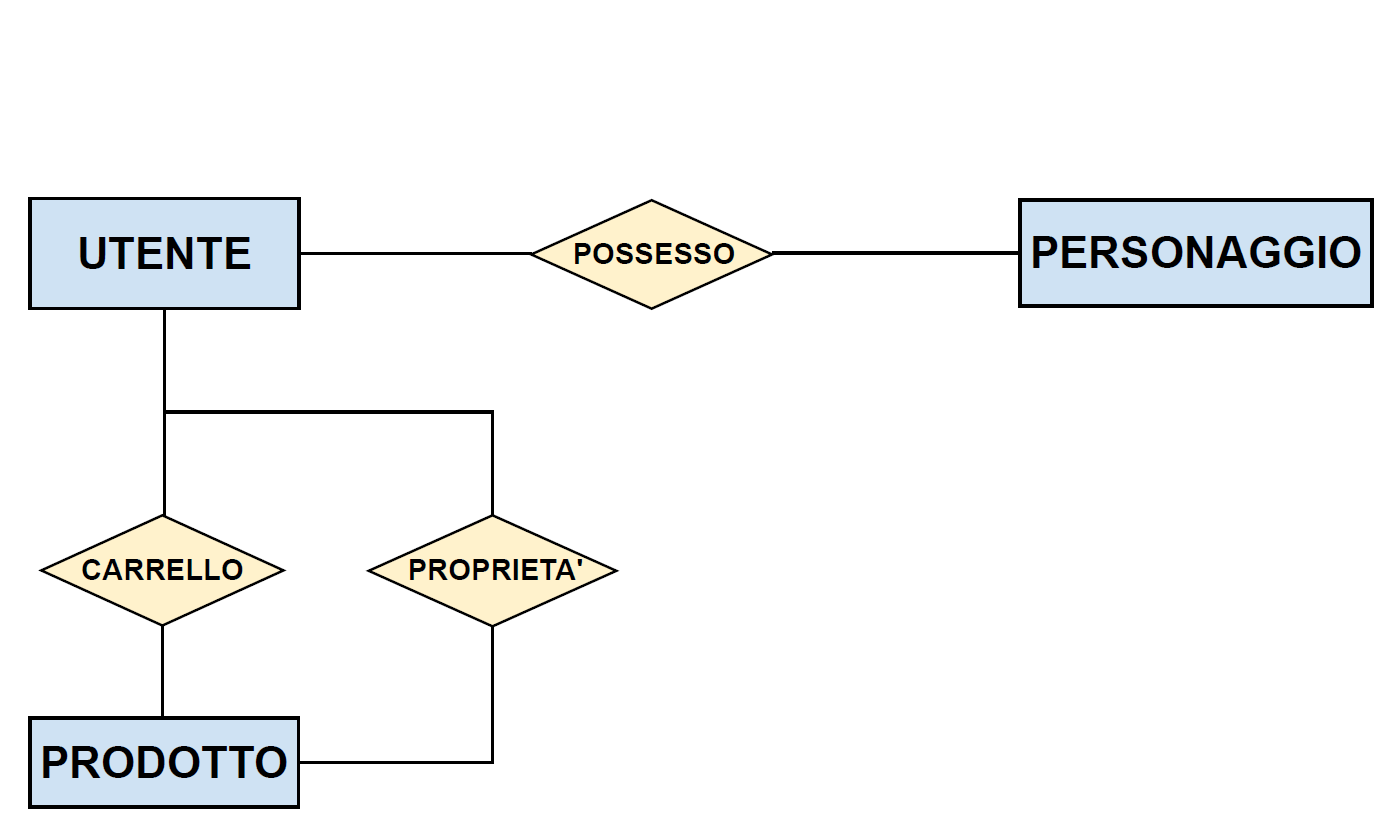
\includegraphics[width=0.7\linewidth]{./immagini/utente.png}
\end{figure}

\newpage